
\section{Assembly Supervisor and State Machine Control}
\label{sec:supervisor}

\subsection{Overview}

The Assembly Supervisor is the central orchestrator of the collaborative robotic assembly system. It implements a robust state machine that governs the complete workflow from task initialization through brick detection, grasp planning, robot coordination, and final assembly placement. This section provides a comprehensive analysis of the supervisor's architecture, state transitions, service and action interactions, and error handling mechanisms that ensure reliable system operation in a collaborative multi-robot environment. An overview of the system-level information flow and control hierarchy is illustrated in Fig.~\ref{fig:assembly_supervisor_architecture}, which shows the interaction between the user interface, perception modules, the Assembly Supervisor, and the two robotic manipulators (AR4 and ABB).

\begin{figure}[H]
    \centering
    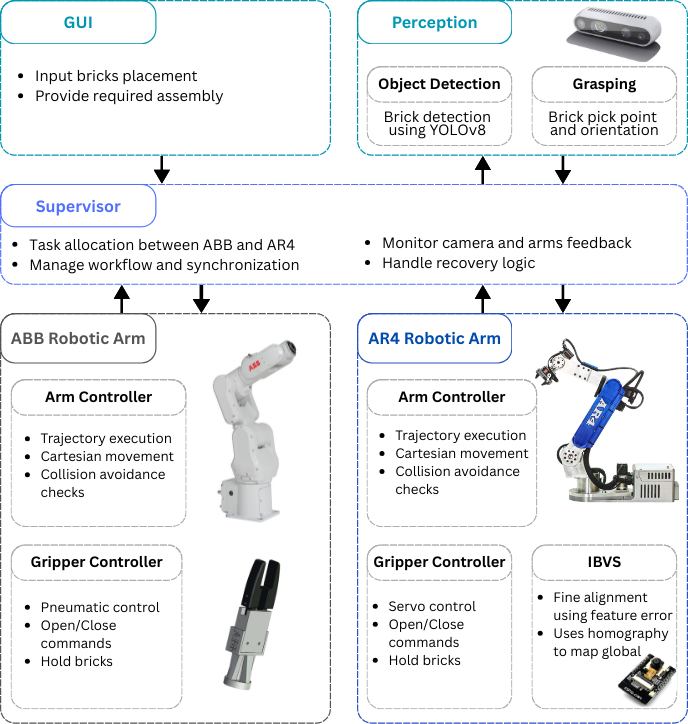
\includegraphics[width=0.85\linewidth]{Figures/chapter3/System_architecture/System.png}
    \caption{High-level architecture of the collaborative assembly system.}
    \label{fig:assembly_supervisor_architecture}
\end{figure}

\subsection{Supervisor Architecture and Responsibilities}

\subsubsection{High-Level Architecture}

The Assembly Supervisor operates as a ROS 2 node with the following core responsibilities:

\begin{itemize}
    \item \textbf{Task Coordination:} Retrieve assembly plans from the GUI and manage task allocation across the two robotic arms.
    \item \textbf{Perception Integration:} Coordinate camera-based brick detection and transform detected poses into the appropriate reference frames.
    \item \textbf{Grasp Inference:} Query the grasp pipeline to select stable grasps for each brick.
    \item \textbf{Motion Execution:} Issue action goals to the AR4 and ABB control servers to execute pick, place, and handover operations.
    \item \textbf{Coordination Logic:} Decide between direct assembly and handover strategies based on brick location and arm allocation.
    \item \textbf{Reference Frame Management:} Transform all detected poses and grasp points into the appropriate coordinate frames using TF2 (ROS 2 Transform Library).
\end{itemize}

\subsubsection{Execution Model and Threading}

The supervisor employs a multi-threaded executor with a \texttt{ReentrantCallbackGroup} to permit concurrent handling of asynchronous ROS 2 callbacks. This design allows:

\begin{itemize}
    \item Parallel service queries and action goal submissions without blocking the main state machine loop.
    \item Safe re-entrant locking when multiple callbacks access shared state variables.
    \item Non-blocking timer-based state machine updates at a controlled frequency (initially 1.0 Hz, reduced to 0.1 Hz during active task execution).
\end{itemize}

\begin{figure}[H]
    \centering
    % \includegraphics[width=0.9\textwidth]{Figures/placeholder_supervisor_architecture}
    \caption{Assembly Supervisor Architecture: Clients, Callbacks, and State Machine}
    \label{fig:supervisor_arch}
\end{figure}

\subsection{ROS 2 Communication: Services and Actions}

\subsubsection{Service Clients}

Services provide synchronous request-response communication for deterministic operations that do not require real-time feedback:

\begin{enumerate}
    \item \textbf{get\_assembly\_plan (Service)}
    \begin{itemize}
        \item \textbf{Purpose:} Retrieve the assembly plan (ordered list of bricks) from the GUI node.
        \item \textbf{Interface:} \texttt{supervisor\_package/srv/GetAssemblyPlan}
        \item \textbf{Response Fields:} Plan array containing brick ID, location, pickup pose, and place pose.
        \item \textbf{Invocation:} Called once during INIT state to bootstrap the assembly sequence.
    \end{itemize}

    \item \textbf{detect\_bricks (Service)}
    \begin{itemize}
        \item \textbf{Purpose:} Trigger YOLOv8 segmentation and brick pose estimation from the global RealSense camera.
        \item \textbf{Interface:} \texttt{dual\_arms\_msgs/srv/DetectBricks}
        \item \textbf{Response Fields:} Array of detected bricks with world poses, plus a computed handover pose (neutral zone between robots).
        \item \textbf{Invocation:} Called during DETECT state to refresh spatial understanding after assembly plan receipt.
    \end{itemize}

    \item \textbf{grasp/get\_grasp\_point (Service)}
    \begin{itemize}
        \item \textbf{Purpose:} Query the transformer-based grasp inference model for the optimal grasp candidate for a specific brick.
        \item \textbf{Interface:} \texttt{dual\_arms\_msgs/srv/GetGrasp}
        \item \textbf{Request Fields:} Brick index (converted to string).
        \item \textbf{Response Fields:} A \texttt{GraspPoint} message containing pose, quality metric, and success indicator.
        \item \textbf{Invocation:} Called for each brick during GRASP\_PIPELINE state before attempting to grasp.
    \end{itemize}
\end{enumerate}

\subsubsection{Action Clients}

Actions provide asynchronous, feedback-capable communication for long-running operations. The supervisor uses action clients to submit motion goals and wait for completion:

\begin{enumerate}
    \item \textbf{ar4\_point\_control (Action)}
    \begin{itemize}
        \item \textbf{Purpose:} Send point-to-point motion commands to the AR4 arm (approach, grasp, release, placement).
        \item \textbf{Interface:} \texttt{supervisor\_package/action/MoveToPose}
        \item \textbf{Goal Fields:} Target pose, strategy (APPROACH\_OFFSET, GRASP, PLACE, \\GOTO\_HANDOVER, RELEASE).
        \item \textbf{Used in States:} EXECUTE\_AR4\_DIRECT, AR4\_PICK\_FOR\_HANDOVER, \\AR4\_PLACE\_ON\_GRID, HANDOVER\_EXECUTION.
    \end{itemize}

    \clearpage

    \item \textbf{ar4\_visual\_servo (Action)}
    \begin{itemize}
        \item \textbf{Purpose:} Execute Image-Based Visual Servoing (IBVS) feedback control via the ESP32-CAM.
        \item \textbf{Interface:} \texttt{supervisor\_package/action/AlignToTarget}
        \item \textbf{Goal Fields:} Object ID (brick type), homography mapping parameters.
        \item \textbf{Behavior:} Iteratively refines AR4 position to align the brick in the ESP32 camera frame, halting once pixel error is below threshold.
        \item \textbf{Used in States:} EXECUTE\_AR4\_DIRECT, AR4\_PICK\_FOR\_HANDOVER.
    \end{itemize}

    \item \textbf{abb\_control (Action)}
    \begin{itemize}
        \item \textbf{Purpose:} Issue high-level task commands to the ABB robot (pick from detected pose, place, pick from handover).
        \item \textbf{Interface:} \texttt{dual\_arms\_msgs/action/ExecuteTask}
        \item \textbf{Goal Fields:} Task type (PICK, PLACE, PICK\_FROM\_HANDOVER), target pose.
        \item \textbf{Behavior:} The ABB controller internally manages gripper open/close, motion planning, and collision avoidance.
        \item \textbf{Used in States:} EXECUTE\_ABB\_PICK, EXECUTE\_ABB\_PLACE, HANDOVER\_EXECUTION.
    \end{itemize}
\end{enumerate}

% \subsubsection{Communication Flow Diagram}

% \begin{figure}[H]
%     \centering
%     % \includegraphics[width=1.0\textwidth]{Figures/placeholder_communication_flow}
%     \caption{Supervisor Service and Action Communication Flow}
%     \label{fig:comm_flow}
% \end{figure}

\subsection{Transform (TF2) Management and Coordinate Frames}

\subsubsection{Coordinate Frame Hierarchy}

The system employs multiple coordinate frames, necessitating careful transformation management:

\begin{itemize}
    \item \textbf{base\_link:} The ABB robot base (designated as the primary world reference frame).
    \item \textbf{camera\_color\_optical\_frame:} The RealSense camera's optical center.
    \item \textbf{ar4\_base:} The AR4 robot's base frame.
    \item \textbf{ar4\_tool:} The AR4 end-effector (gripper) frame.
    \item \textbf{esp32\_cam\_optical:} The ESP32-CAM's optical frame (eye-in-hand).
    \item \textbf{table:} A virtual frame representing the assembly table surface.
\end{itemize}

\subsubsection{Transform Pipeline}

The supervisor uses TF2 to establish and maintain transformations:

\begin{enumerate}
    \item \textbf{Brick Detection to World Frame:}
    \begin{itemize}
        \item Input: Brick pose in \texttt{camera\_color\_optical\_frame} from YOLOv8 segmentation.
        \item Transformation: \texttt{lookup\_transform('base\_link', 'camera\_color\_optical\_frame')}
        \item Output: Brick pose in \texttt{base\_link} (ABB world frame) for unified task planning.
    \end{itemize}

    \item \textbf{Grasp Point Transformation:}
    \begin{itemize}
        \item The grasp pipeline returns a \texttt{GraspPoint} in the camera frame.
        \item The supervisor applies the same camera-to-base transformation.
        \item Additional adjustments are made: Z-coordinate clamped to safety height (0.22 m), orientation components reordered to match AR4 conventions.
    \end{itemize}

    \item \textbf{Handover Pose Transformation:}
    \begin{itemize}
        \item The global detection service computes a handover pose (midpoint between the two robots).
        \item The supervisor transforms this pose to \texttt{base\_link} for consistency.
    \end{itemize}
\end{enumerate}

\subsubsection{Transform Implementation Details}

The supervisor implements transform lookups with error handling. A typical lookup operation:

\begin{verbatim}
def transform_pose_to_abb(self, input_pose):
    try:
        t = self.tf_buffer.lookup_transform(
            'base_link', 
            'camera_color_optical_frame', 
            rclpy.time.Time())
        transformed_pose = tf2_geometry_msgs.do_transform_pose(
            input_pose, t)
        return transformed_pose
    except TransformException as ex:
        self.get_logger().error(f'TF2 Error: {ex}')
        return input_pose  # Fallback
\end{verbatim}

This implementation:
\begin{itemize}
    \item Uses \texttt{rclpy.time.Time()} to request the latest available transform.
    \item Falls back to the original pose if transformation fails (avoiding system crash).
    \item Logs transformation errors for debugging.
\end{itemize}

% \begin{figure}[H]
%     \centering
%     % \includegraphics[width=0.9\textwidth]{Figures/placeholder_tf_hierarchy}
%     \caption{Coordinate Frame Hierarchy and Transform Chain}
%     \label{fig:tf_hierarchy}
% \end{figure}

\subsection{Detailed State Machine Analysis}

\subsubsection{State Machine Overview}

The Assembly Supervisor implements a 12-state finite state machine that governs the complete assembly workflow. States are organized into five logical stages:

\begin{enumerate}
    \item \textbf{Stage 1 - Initialization (INIT):} Retrieve assembly plan and validate input.
    \item \textbf{Stage 2 - Perception (DETECT):} Obtain global brick poses and compute handover zone.
    \item \textbf{Stage 3 - Task Allocation (PROCESS\_NEXT, GRASP\_PIPELINE):} Select next brick and compute grasp.
    \item \textbf{Stage 4 - Execution (Multiple states):} Execute grasping, handover, or placement based on allocation.
    \item \textbf{Stage 5 - Termination (DONE):} All tasks complete; system idle.
\end{enumerate}

\begin{figure}[H]
    \centering
    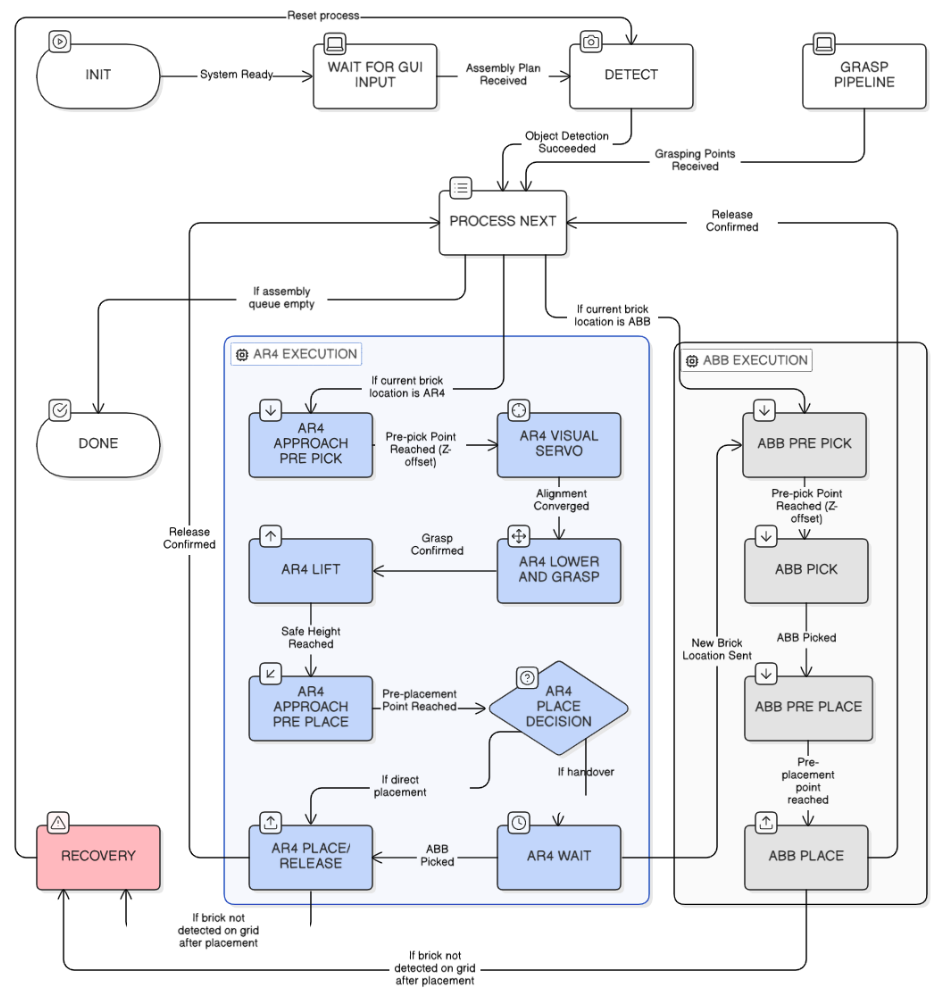
\includegraphics[width=0.75\textwidth]{Figures/chapter3/Supervisor/States.png}
    \caption{Complete State Machine Diagram with Transitions}
    \label{fig:state_machine_diagram}
\end{figure}

\subsubsection{State 1: INIT (Initialization)}
\label{state:init}

\paragraph{Purpose}

Retrieve the assembly plan from the GUI and bootstrap the state machine. This state validates that a plan is available before proceeding to perception.

\paragraph{Execution Logic}

\begin{enumerate}
    \item Check if the \texttt{gui\_client} service is available using \texttt{wait\_for\_service(timeout\_sec=1.0)}.
    \item If unavailable, log a message and reschedule the state machine loop after a 2-second delay.
    \item If available, submit a \texttt{GetAssemblyPlan} service request (empty request body).
    \item Validate the response: Check that \texttt{result.plan} is not \texttt{None} and contains at least one brick.
    \item On valid plan receipt, store plan in \texttt{self.assembly\_queue} and transition to DETECT.
    \item On invalid plan, log a warning and reschedule after 2 seconds (remain in INIT).
\end{enumerate}

\paragraph{Error Handling}

\begin{itemize}
    \item \textbf{Service Not Ready:} Reschedule and wait. This handles GUI node startup delays.
    \item \textbf{Empty Plan:} Log and retry. This distinguishes between ``service not ready'' and ``no plan available''.
    \item \textbf{Network Failure:} Timeout on \texttt{wait\_for\_service} is caught; state remains INIT.
\end{itemize}

\paragraph{Transition}

\begin{itemize}
    \item Success: INIT $\rightarrow$ DETECT
    \item Retry: INIT $\rightarrow$ INIT (after 2 seconds)
\end{itemize}

\subsubsection{State 2: DETECT (Global Perception)}
\label{state:detect}

\paragraph{Purpose}

Invoke YOLOv8 segmentation and pose estimation to obtain brick positions in the global camera frame. Transform all poses to the ABB base frame.

\paragraph{Execution Logic}

\begin{enumerate}
    \item Check service availability: \texttt{self.camera\_client.wait\_for\_service(timeout\_sec=1.0)}.
    \item If unavailable, log error and reschedule.
    \item Submit a \texttt{DetectBricks} service request.
    \item Receive response containing:
    \begin{itemize}
        \item \texttt{result.bricks[*]:} Array of detected bricks with pose in camera frame.
        \item \texttt{result.handover\_pose:} Computed neutral zone pose in camera frame.
    \end{itemize}
    \item For each brick, apply transform: \texttt{brick.pose = self.transform\_pose\_to\_abb(brick.pose)}.
    \item Similarly, transform handover pose: \texttt{self.handover\_pose = self.transform\_pose\_to\_abb(result.handover\_pose)}.
    \item Store transformed bricks in \texttt{self.detected\_bricks}.
    \item Transition to PROCESS\_NEXT.
\end{enumerate}

\paragraph{Pose Validation}

After transformation, poses are validated:
\begin{itemize}
    \item Z-coordinate should be non-negative (on or above table).
    \item X, Y coordinates should be within workspace bounds.
    \item Orientation quaternion should be normalized.
\end{itemize}

\paragraph{Transition}

\begin{itemize}
    \item Success: DETECT $\rightarrow$ PROCESS\_NEXT
\end{itemize}

\subsubsection{State 3: PROCESS\_NEXT (Task Dequeue)}
\label{state:processnext}

\paragraph{Purpose}

Remove the next brick from the assembly queue and initiate grasp planning. This state acts as a checkpoint for per-brick initialization.

\paragraph{Execution Logic}

\begin{enumerate}
    \item Check if \texttt{self.assembly\_queue} is empty.
    \item If empty: transition to DONE and exit.
    \item If non-empty: pop the first element and assign to \texttt{self.current\_brick}.
    \item Transition to GRASP\_PIPELINE.
\end{enumerate}

\paragraph{Transition}

\begin{itemize}
    \item Bricks remaining: PROCESS\_NEXT $\rightarrow$ GRASP\_PIPELINE
    \item No bricks: PROCESS\_NEXT $\rightarrow$ DONE
\end{itemize}

\subsubsection{State 4: GRASP\_PIPELINE (Grasp Inference)}
\label{state:grasppipeline}

\paragraph{Purpose}

Query the transformer-based grasp inference model to obtain a stable grasp candidate for the current brick. Apply pose transformation and additional safety adjustments.

\paragraph{Execution Logic}

\begin{enumerate}
    \item Check service availability: \texttt{self.grasp\_pipeline\_client.wait\_for\_service(timeout\_sec=2.0)}.
    \item If unavailable, log error, transition to PROCESS\_NEXT (skip brick), and return.
    \item Create a \texttt{GetGrasp.Request()} with \texttt{brick\_index = str(self.current\_brick.id)}.
    \item Submit request asynchronously and await response.
    \item Check \texttt{grasp\_result.success} flag:
    \begin{itemize}
        \item If True: Extract \texttt{grasp\_result.grasp\_point} (a \texttt{GraspPoint} message).
        \item If False: Log error, transition to PROCESS\_NEXT, skip brick.
    \end{itemize}
    \item Apply coordinate frame transformation.
    \item Apply safety adjustments (clamp Z-coordinate, reorder orientation).
    \item Store transformed grasp in \texttt{self.current\_grasp\_point}.
    \item Determine arm allocation based on \texttt{self.current\_brick.location}.
\end{enumerate}

\paragraph{Grasp Point Structure}

The \texttt{GraspPoint} message contains:
\begin{verbatim}
geometry_msgs/Pose pose          # Grasp position and orientation
float32 quality                  # Quality metric [0, 1]
float32 width                    # Finger opening distance (meters)
float32 approach_angle           # Recommended approach angle (radians)
\end{verbatim}

\paragraph{Arm Allocation Logic}

Based on brick location from the assembly plan:
\begin{itemize}
    \item \texttt{location == 1:} Brick on ABB's side $\rightarrow$ EXECUTE\_ABB\_PICK
    \item \texttt{location == 2:} Brick requires handover $\rightarrow$ HANDOVER\_SEQUENCE
    \item Other: Brick on AR4's side $\rightarrow$ EXECUTE\_AR4\_DIRECT
\end{itemize}

\paragraph{Transition}

\begin{itemize}
    \item Grasp success, ABB-side brick: GRASP\_PIPELINE $\rightarrow$ EXECUTE\_ABB\_PICK
    \item Grasp success, AR4-side brick: GRASP\_PIPELINE $\rightarrow$ EXECUTE\_AR4\_DIRECT
    \item Grasp success, handover-required: GRASP\_PIPELINE $\rightarrow$ HANDOVER\_SEQUENCE
    \item Grasp failure: GRASP\_PIPELINE $\rightarrow$ PROCESS\_NEXT
\end{itemize}

\subsubsection{State 5: EXECUTE\_AR4\_DIRECT (AR4 Pick and Place)}
\label{state:executeAR4direct}

\paragraph{Purpose}

Execute a complete pick-and-place cycle using the AR4 robot for bricks allocated to the AR4's workspace.

\paragraph{Sub-Step A: Approach with Offset}

\begin{enumerate}
    \item Create a \texttt{MoveToPose} action goal with strategy ``APPROACH\_OFFSET''.
    \item The AR4 controller offsets in the approach direction to maintain safe clearance.
    \item Await completion.
\end{enumerate}

\paragraph{Sub-Step B: Visual Servoing (IBVS)}

\begin{enumerate}
    \item Create an \texttt{AlignToTarget} action goal with object ID and homography parameters.
    \item The visual servoing action server:
    \begin{itemize}
        \item Captures images from the ESP32-CAM.
        \item Detects the brick and computes image-space error.
        \item Uses IBVS feedback law to generate AR4 velocity commands.
        \item Continues until error is below threshold.
    \end{itemize}
    \item Await completion.
\end{enumerate}

\paragraph{Sub-Step C: Grasp and Retract}

\begin{enumerate}
    \item Create a \texttt{MoveToPose} action goal with strategy ``GRASP''.
    \item The AR4 controller executes final approach and closes the gripper.
    \item Await completion.
\end{enumerate}

\paragraph{Transition}

\begin{itemize}
    \item Success: EXECUTE\_AR4\_DIRECT $\rightarrow$ AR4\_PLACE\_ON\_GRID
\end{itemize}

\subsubsection{State 6: AR4\_PLACE\_ON\_GRID (AR4 Placement)}
\label{state:ar4place}

\paragraph{Purpose}

Move the grasped brick to the assembly grid location specified by the plan.

\paragraph{Execution Logic}

\begin{enumerate}
    \item Create a \texttt{MoveToPose} action goal with strategy ``PLACE''.
    \item Submit to AR4 point control action server.
    \item The AR4 controller moves and opens the gripper.
    \item Await completion.
    \item Transition to PROCESS\_NEXT.
\end{enumerate}

\paragraph{Transition}

\begin{itemize}
    \item Success: AR4\_PLACE\_ON\_GRID $\rightarrow$ PROCESS\_NEXT
\end{itemize}

\subsubsection{State 7: EXECUTE\_ABB\_PICK (ABB Grasping)}
\label{state:executeABBpick}

\paragraph{Purpose}

Execute pick operation using the ABB robot for bricks on the ABB's side of the workspace.

\paragraph{Execution Logic}

\begin{enumerate}
    \item Create an \texttt{ExecuteTask} action goal with task type ``PICK''.
    \item Submit to ABB control action server.
    \item The ABB controller plans and executes the pick sequence.
    \item Await completion.
    \item Transition to EXECUTE\_ABB\_PLACE.
\end{enumerate}

\paragraph{Transition}

\begin{itemize}
    \item Success: EXECUTE\_ABB\_PICK $\rightarrow$ EXECUTE\_ABB\_PLACE
\end{itemize}

\subsubsection{State 8: EXECUTE\_ABB\_PLACE (ABB Placement)}
\label{state:executeABBplace}

\paragraph{Purpose}

Place the grasped brick at its designated location on the assembly grid.

\paragraph{Execution Logic}

\begin{enumerate}
    \item Create an \texttt{ExecuteTask} action goal with task type ``PLACE''.
    \item Apply safety adjustment: Set Z-coordinate to 0.24 m.
    \item Submit to ABB control action server.
    \item Await completion.
    \item Transition to PROCESS\_NEXT.
\end{enumerate}

\paragraph{Transition}

\begin{itemize}
    \item Success: EXECUTE\_ABB\_PLACE $\rightarrow$ PROCESS\_NEXT
\end{itemize}

\subsubsection{State 9: HANDOVER\_SEQUENCE (Handover Initiation)}
\label{state:handoversequence}

\paragraph{Purpose}

Transition to handover workflow when a brick must be transferred from AR4 to ABB.

\paragraph{Execution Logic}

\begin{enumerate}
    \item This state is a pass-through (no action).
    \item Immediately transition to AR4\_PICK\_FOR\_HANDOVER.
\end{enumerate}

\paragraph{Transition}

\begin{itemize}
    \item HANDOVER\_SEQUENCE $\rightarrow$ AR4\_PICK\_FOR\_HANDOVER
\end{itemize}

\subsubsection{State 10: AR4\_PICK\_FOR\_HANDOVER (AR4 Grasping for Transfer)}
\label{state:ar4pickhandover}

\paragraph{Purpose}

Execute the AR4 grasping sequence in preparation for handover.

\paragraph{Execution Logic}

See Sub-Steps A, B, C under State 5 (EXECUTE\_AR4\_DIRECT).

\paragraph{Transition}

\begin{itemize}
    \item Success: AR4\_PICK\_FOR\_HANDOVER $\rightarrow$ HANDOVER\_EXECUTION
\end{itemize}

\subsubsection{State 11: HANDOVER\_EXECUTION (Coordinated Transfer)}
\label{state:handoverexecution}

\paragraph{Purpose}

Execute synchronized handover between the AR4 and ABB robots.

\paragraph{Step 1: AR4 Move to Handover Zone}

\begin{enumerate}
    \item Create a \texttt{MoveToPose} action goal with strategy ``GOTO\_HANDOVER''.
    \item Submit to AR4 point control action server.
    \item Await completion.
\end{enumerate}

\paragraph{Step 2: ABB Approach and Grasp}

\begin{enumerate}
    \item Create an \texttt{ExecuteTask} action goal with task type ``PICK\_FROM\_HANDOVER''.
    \item Submit to ABB control action server.
    \item The ABB controller approaches and closes gripper.
    \item Await completion.
\end{enumerate}

\paragraph{Step 3: AR4 Release}

\begin{enumerate}
    \item Create a \texttt{MoveToPose} action goal with strategy ``RELEASE''.
    \item Submit to AR4 point control action server.
    \item The AR4 controller opens gripper and retracts.
    \item Await completion.
\end{enumerate}

\paragraph{Transition}

\begin{itemize}
    \item Success: HANDOVER\_EXECUTION $\rightarrow$ PROCESS\_NEXT
\end{itemize}

\paragraph{Handover Synchronization Considerations}

\begin{itemize}
    \item \textbf{Sequential Approach:} Strict sequential steps ensure clear state and avoid conflicts.
    \item \textbf{Force Feedback (Future):} Force/torque sensors could enable simultaneous dual-robot grasp confirmation.
    \item \textbf{Fallback Strategy:} If ABB grasp fails, AR4 does not release; system can retry.
\end{itemize}

\subsubsection{State 12: DONE (Completion)}
\label{state:done}

\paragraph{Purpose}

Signal that all tasks are completed and the system is idle.

\paragraph{Execution Logic}

\begin{enumerate}
    \item Log completion message.
    \item Do not reschedule the state machine loop timer.
    \item System waits for external INIT signal or restart.
\end{enumerate}

\paragraph{Transition}

\begin{itemize}
    \item DONE $\rightarrow$ (Await external signal)
\end{itemize}

\subsection{Error Handling and Recovery}

\subsubsection{Service Availability Checking}

The supervisor checks service availability before submitting requests. If unavailable:
\begin{itemize}
    \item Log a diagnostic message.
    \item Reschedule the state machine loop after a delay (2 seconds).
    \item Remain in current state, retrying the same action.
\end{itemize}

\subsubsection{Action Goal Failure}

When an action goal is rejected:
\begin{itemize}
    \item Check the goal handle status.
    \item Log an error and return False.
    \item The calling state decides on recovery (retry or skip).
\end{itemize}

\subsubsection{Transform Lookup Failures}

If a TF2 transform is unavailable:
\begin{itemize}
    \item Catch \texttt{TransformException}.
    \item Log the exception.
    \item Return the original pose as fallback.
\end{itemize}

\subsubsection{Grasp Pipeline Failures}

If the grasp service returns \texttt{success=False}:
\begin{itemize}
    \item Log the failure.
    \item Transition to PROCESS\_NEXT (skip the brick).
\end{itemize}

\subsubsection{Robot Timeout}

If an action goal does not complete within a reasonable time:
\begin{itemize}
    \item Cancel the goal and log the failure.
    \item Transition to PROCESS\_NEXT.
    \item Proceed with the next brick.
\end{itemize}

\subsection{Concurrency and Threading Model}

\subsubsection{ReentrantCallbackGroup}

The supervisor uses \texttt{ReentrantCallbackGroup} to allow concurrent callback execution:
\begin{itemize}
    \item Asynchronous service responses processed during state machine operation.
    \item Non-blocking behavior for long-running actions.
\end{itemize}

\subsubsection{MultiThreadedExecutor}

The supervisor node uses \texttt{MultiThreadedExecutor}:
\begin{itemize}
    \item Allocates thread pool for callback handling.
    \item Async/await patterns execute without blocking.
    \item Safe re-entrant locking for shared state.
\end{itemize}

\subsubsection{Potential Race Conditions}

\begin{itemize}
    \item \textbf{assembly\_queue modification:} Mitigated by single-threaded state machine logic.
    \item \textbf{current\_brick and grasp data:} Protected by sequential state transitions.
    \item \textbf{detected\_bricks refresh:} Snapshot consistency assumed.
\end{itemize}

\subsection{State Machine Timing and Scheduling}

\subsubsection{Timer Management}

The supervisor uses \texttt{rclpy.time.Timer} for periodic state machine invocations:
\begin{itemize}
    \item \textbf{Initialization:} Timer created at 1.0 Hz frequency.
    \item \textbf{Dynamic Frequency:} Reset to 0.1 Hz during heavy computation to reduce CPU overhead.
    \item \textbf{Cancellation:} Timer canceled when state machine completes or encounters blocking actions.
\end{itemize}

\subsubsection{Async/Await Pattern}

The state machine loop is asynchronous, enabling:
\begin{itemize}
    \item Non-blocking waiting for service responses.
    \item Clean exception handling and state transitions.
    \item Delayed task scheduling and timer rescheduling.
\end{itemize}

\subsection{Hardware and Sensor Integration}

\subsubsection{Robotic Arms}

\paragraph{ABB Robot}
\begin{itemize}
    \item \textbf{Model:} IRB 1200-5/90 (industrial manipulator).
    \item \textbf{Workspace:} Covers placement side of assembly table.
    \item \textbf{Gripper:} Two-finger parallel gripper.
    \item \textbf{Communication:} ROS 2 action server at \texttt{abb\_control}.
    \item \textbf{Payload Capacity:} Sufficient for single brick grasping.
\end{itemize}

\paragraph{AR4 Robot}
\begin{itemize}
    \item \textbf{Model:} Annin Robotics AR4 (4-DOF SCARA-style arm).
    \item \textbf{Workspace:} Covers grasping/pickup side.
    \item \textbf{Gripper:} Two-finger gripper controlled via ESP32.
    \item \textbf{Eye-in-Hand Camera:} ESP32-CAM for local perception.
    \item \textbf{Communication:} ROS 2 action servers at \texttt{ar4\_point\_control} and \texttt{ar4\_visual\_servo}.
    \item \textbf{Calibration:} Position correction via polynomial regression (Section~\ref{sec:ar4_calibration}).
\end{itemize}

\subsubsection{Cameras and Perception}

\paragraph{Intel RealSense D435i (Global Perception)}
\begin{itemize}
    \item \textbf{Placement:} Fixed above assembly table covering full workspace.
    \item \textbf{Output:} RGB images for YOLOv8 segmentation.
    \item \textbf{Calibration:} Camera-to-ABB-base transformation in TF2.
    \item \textbf{Update Rate:} 30 Hz.
\end{itemize}

\paragraph{ESP32-CAM (Eye-in-Hand Perception)}
\begin{itemize}
    \item \textbf{Placement:} Mounted on AR4 end-effector.
    \item \textbf{Output:} Low-resolution RGB for feature detection and visual servoing.
    \item \textbf{Calibration:} Homography mapping from RealSense to ESP32 view.
    \item \textbf{Update Rate:} 5--10 Hz.
    \item \textbf{Latency:} 100--200 ms (mitigated by low-gain feedback control).
\end{itemize}

\subsection{Data Flow and Message Passing}

\subsubsection{Brick Representation}

The system represents bricks with the following structure:
\begin{verbatim}
dual_arms_msgs/Brick:
  int32 id                    # Unique identifier
  int32 type                  # Brick class
  int32 location              # 1=ABB side, 2=Handover, other=AR4
  geometry_msgs/Pose pickup_pose
  geometry_msgs/Pose place_pose
\end{verbatim}

\subsubsection{Grasp Point Representation}

Grasp candidates are represented as:
\begin{verbatim}
dual_arms_msgs/GraspPoint:
  geometry_msgs/Pose pose     # Position and orientation
  float32 quality             # Metric [0, 1]
  float32 width               # Finger opening [meters]
  float32 approach_angle      # Approach direction
\end{verbatim}

\subsection{Debugging and Logging}

\subsubsection{Log Levels}

The supervisor uses ROS 2 logging with different verbosity levels:
\begin{itemize}
    \item \textbf{INFO:} State transitions, service calls, task completion.
    \item \textbf{WARN:} Empty plans, service delays, non-critical failures.
    \item \textbf{ERROR:} Service unavailability, transform failures, action rejections.
\end{itemize}

\subsubsection{State Machine Monitoring}

Current logging provides visibility into:
\begin{itemize}
    \item State transitions.
    \item Task counts.
    \item Brick-specific progress.
    \item Grasp quality metrics.
\end{itemize}

\subsection{Summary}

The Assembly Supervisor implements a robust, multi-threaded state machine that orchestrates a collaborative two-robot assembly system. Key features include:

\begin{enumerate}
    \item \textbf{Modular Service/Action Architecture:} Clean separation between perception, execution, and decision logic.
    \item \textbf{Transform Management:} Consistent use of TF2 for coordinate frame conversions.
    \item \textbf{Comprehensive State Machine:} 12 states covering all operational phases with clear error recovery paths.
    \item \textbf{Concurrency Support:} MultiThreadedExecutor enables responsive, non-blocking operation.
    \item \textbf{Hardware Integration:} Direct control of two heterogeneous arms with different control models.
    \item \textbf{Error Resilience:} Timeouts, service failures, and inference failures handled gracefully.
\end{enumerate}

The supervisor's structured approach provides a foundation for reliable, repeatable collaborative assembly operations and facilitates integration with the Digital Twin for monitoring and optimization.